%%
%%H27年度情報工学科卒業研究概要スタイルファイル
%%
\documentclass[a4j,twoside]{jarticle}
\usepackage[dvipdfmx]{graphicx}
\usepackage{thesis_abst}
\usepackage{here}

%マージンはプリンタによって変更
\addtolength{\oddsidemargin}{0mm}
\addtolength{\evensidemargin}{0mm}

%baselinestretchを変更すると上部枠の大きさが変わるのでおすすめしない
\renewcommand{\baselinestretch}{1}

\種別{情 報 工 学 科 卒 業}  %この行を消してはいけない
%\種別{電 気 情 報 工 学 科 卒 業}  %電気情報1,2部の人はこちらを生かす。
\学籍番号{24115113}
\氏名{林 政行}
%\英語氏名{} %未使用
\研究室{伊藤孝行} % 所属する研究室名
\系{知能} % 学生が所属する系を記入.教員(研究室)の所属する系ではない
%           電情の学生のように「系」がないときは、この行をコメントに。
\題目{降水量予測のための\\{\small Sequence-to-Sequence}モデルに基づくマルチモーダル学習} % 途中で改行 "\\" を挿入可
\年度{27} % !=年 発表は2月です

\begin{document}			%この行を消してはいけない
\twocolumn[\vspace*{9mm}]	%この行を消してはいけない
\begin{論文概要}				%この行を消してはいけない
\setcounter{page}{1}		%表(左綴じ)は1、裏(右綴じ)は2を指定
%%%%%%% ここからアブスト本体 %%%%%%%
\section{はじめに}
%
集中豪雨による災害を未然に防ぐために,5分後から6時間後といった近い将来の高精度な降水量の予測が求められている.

降水量は気象レーダーにより観測され,格子状に値が入ったレーダーマップとして得られる.
既存手法として,機械学習の手法により降水量予測を行う{\small Convolutional LSTM Sequence to Sequence}モデル(ConvLSTM-seq2seq)が提案されている\cite{shi2015convolutional}.
%ConvLSTM-seq2seqでは,降水量予測の問題を,過去の連続的に観測されたレーダーマップを入力し,引き続く将来の連続的なレーダーマップを出力する,時空間データの予測問題と捉え,ConvLSTMという拡張したLSTMをSequence to Sequence学習フレームワーク\cite{sutskever2014sequence}において用いることで解いている.
%ConvLSTM-seq2seqでは,降水量予測の問題を,過去の連続的に観測されたレーダーマップを入力し,引き続く将来の連続的なレーダーマップを出力する,時空間データの予測問題と捉え,ConvLSTMという拡張したLSTMを深層学習のSequence to Sequence (seq2seq) 学習フレームワークにおいて用いることで解いている.
ConvLSTM-seq2seqでは,降水量予測の問題を,過去の連続的なレーダーマップを入力し,引き続く将来の連続的なレーダーマップを出力する,時空間データの予測問題と捉え,ConvLSTMという拡張したLSTMを深層学習のSequence to Sequence (seq2seq) 学習フレームワークにおいて用いることで解いている.

しかし,将来の降水量は風向きや地形といった複数の要因(モダリティ)に依存するが,既存手法では過去の降水量のみが予測に用いられている.
そこで本研究では,ConvLSTM-seq2seqにマルチモーダル学習を取り入れ,過去に観測された複数のモダリティから将来の降水量の予測を行う,時空間データのマルチモーダル学習手法を提案する.

%深層学習におけるマルチモーダル学習の手法として,Andrewらにより,正準相関分析(Canonical Correlation Analysis; CCA)を取り入れたDeep CCA (DCCA)が提案されている\cite{andrew2013deep}.
%
\section{{\normalsize 時空間データのマルチモーダル学習手法の提案}}
\label{model:chapter}
%
%提案する手法は,複数モダリティの多チャンネル画像入力による手法と正準相関分析を取り入れた手法の2つである.
\subsection{提案手法1: 多チャンネル画像入力による手法}
%
マルチモーダル学習を実現する最も簡単な方法として,2次元画像として扱われる各モダリティを結合し,多チャンネルから成る画像としてConvLSTMに入力する手法を提案する.
%
\subsection{提案手法2: 正準相関分析を取り入れた手法}
Andrewらにより,深層学習におけるマルチモーダル学習手法として正準相関分析(Canonical Correlation Analysis; CCA)を取り入れたDeep CCA (DCCA)が提案されている\cite{andrew2013deep}.
本研究ではConvLSTM-seq2seqにDCCAを取り入れマルチモーダル学習を行う手法を提案する.
\begin{figure}[b]
	%\vspace{-0.28cm}
	\centering
	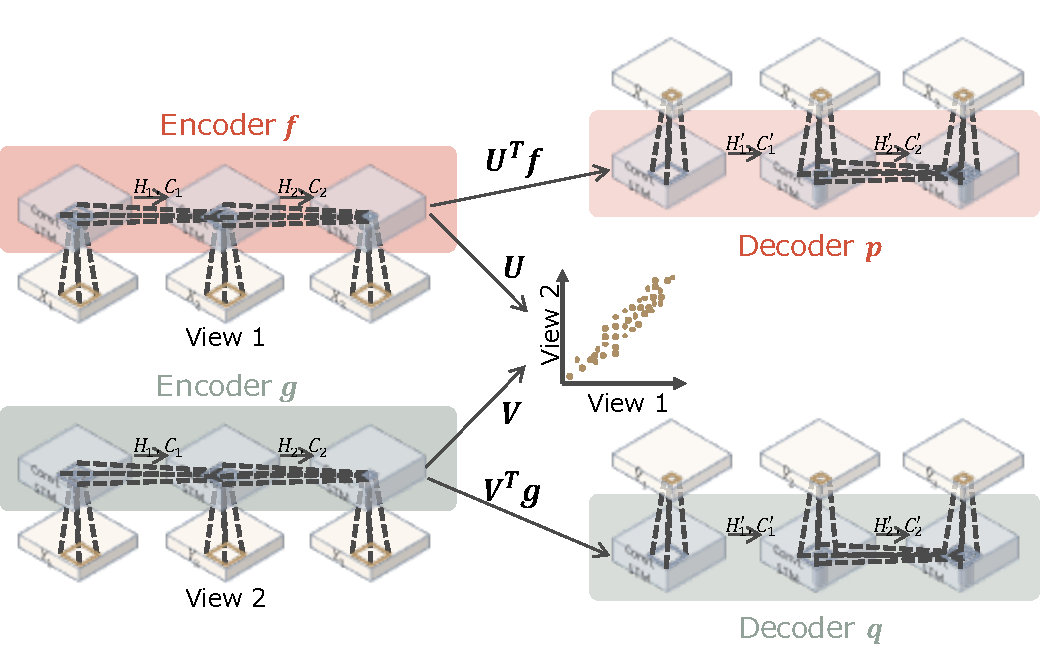
\includegraphics[width=5.6cm]{../images/3.The_Model/the_model_dcca_pretrain.pdf}
	\vspace{-0.28cm}
	\caption{提案手法2}
	\label{fig:the_model_dcca_pretrain}
	%\vspace{-0.25cm}
\end{figure} 
%提案手法では,seq2seqモデルにおいて,入力するモダリティごとに異なるエンコーダを用い,エンコーダにより得られた各モダリティの表現についてCCAを適用する.
%CCAはAutoencoderネットワークにより入力の復元を行う事前学習に取り入れられ,事前学習の後,目標出力を出力するようさらに学習(finetune)を行う.
図\ref{fig:the_model_dcca_pretrain}に示す提案手法では,seq2seqモデルにおいて,入力するモダリティごとに異なるエンコーダを用い,エンコーダの最後のタイムステップにおけるConvLSTMの状態を表現として捉え,各モダリティについて得られた表現にCCAを適用する.
%
\section{降水量予測タスクによる評価実験}
%
評価実験では愛知県を中心とした観測領域について5分間隔で観測された,レーダーマップと衛星画像の2つのモダリティを用いて,降水量予測を行った.
%実験設定として,$45,40,...,0$分前の観測値10フレームを入力し,$5,10,...,50$分後の予測値(レーダーマップ)10フレームを出力する問題とし,出力と目標との誤差関数には交差エントロピー誤差を用いた.
実験設定として,$45,40,...,0$分前の観測値10フレームを入力し,$5,10,...,50$分後の予測値10フレームを出力する問題とした.
%既存手法はConvLSTM-seq2seqによりレーダー観測値のみを予測に用いる単一モーダル学習を指す.
%提案手法は\ref{model:chapter}章で述べたマルチモーダル学習手法を指す.
\begin{figure}[h]
	\centering
	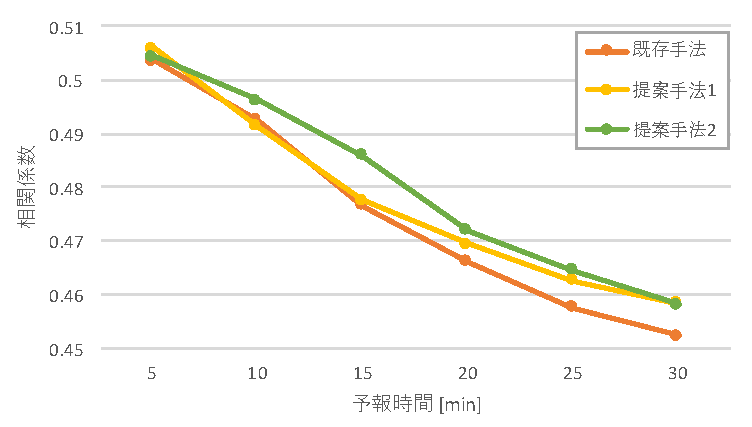
\includegraphics[width=6.3cm]{../images/5.Experiment/exp2_correlation_abst.pdf}
	\vspace{-0.2cm}
	\caption{実験結果: 予測系列の前半6フレームの相関}
	\label{fig:exp_correlation}
	\vspace{-0.1cm}
\end{figure}
%\begin{figure}[h]
%	\centering
%	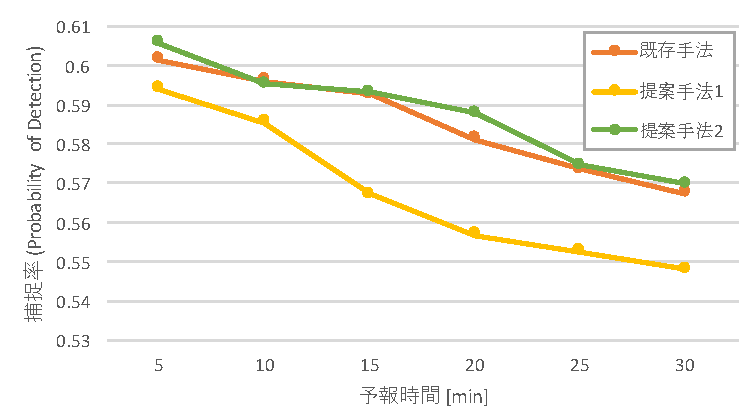
\includegraphics[width=6.3cm]{../images/5.Experiment/exp2_pod_abst.pdf}
%	\vspace{-0.2cm}
%	\caption{実験結果: 予測系列の前半6フレームの捕捉率}
%	\label{fig:exp_correlation}
%	\vspace{-0.1cm}
%\end{figure}
\begin{figure}[h]
	%\vspace{-0.4cm}
	\centering
	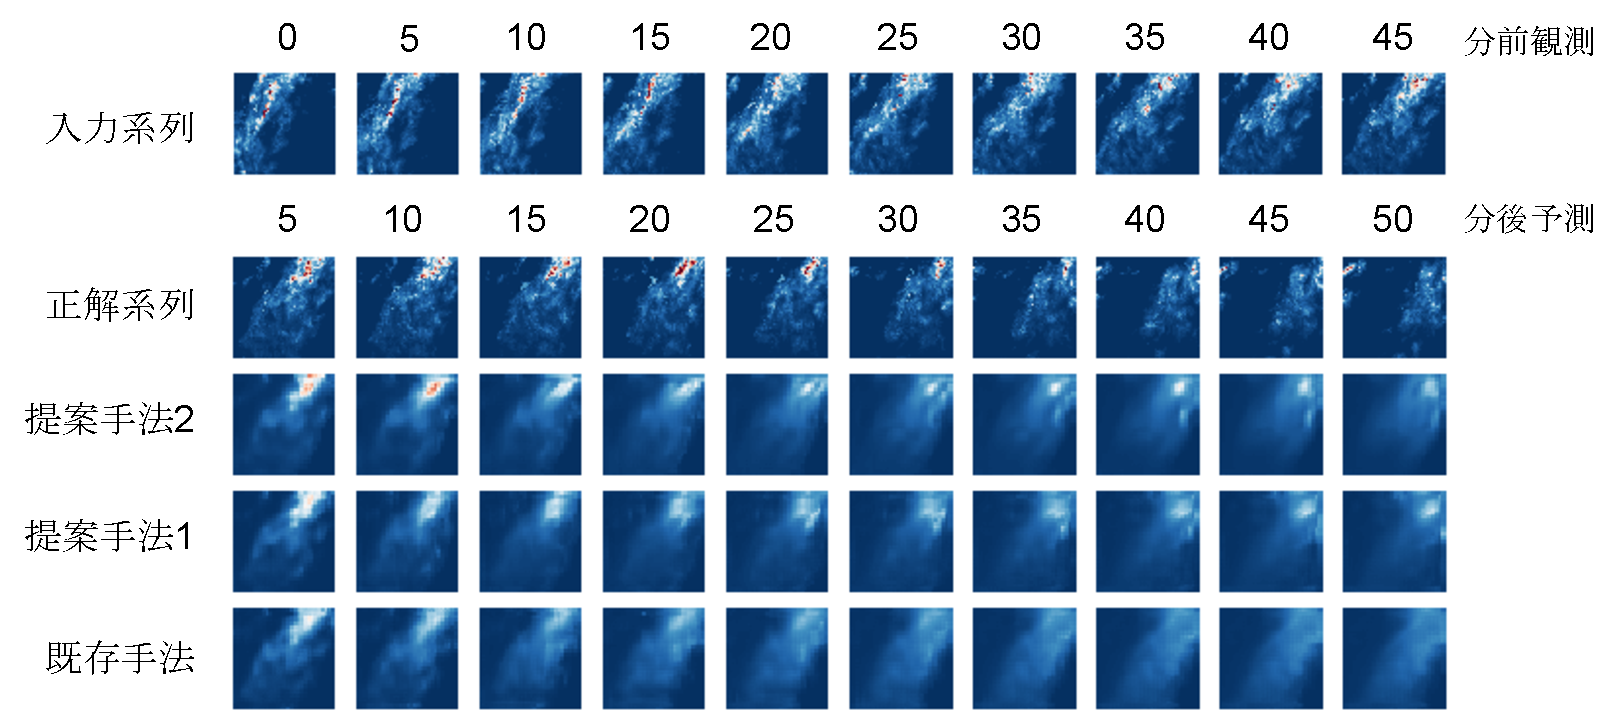
\includegraphics[width=8cm]{../images/5.Experiment/xxx-merged-473-c.pdf}
	\caption{実験結果: 予測系列の例}
	\label{fig:the_model_dcca}
	%\vspace{-0.4cm}
\end{figure}
図\ref{fig:exp_correlation}に予測フレームごとの正解値と予測値との相関係数を示す.
%図\ref{fig:exp_correlation}に予測フレームごとの各手法での捕捉率を示す.
また,図\ref{fig:exp_correlation}に予測結果の一例を示す.
実験結果より,5分後から30分後の短時間の降水量予測について,提案手法2が既存手法を上回る精度で予測できることを確認した.
%実験結果より,5分後から30分後の短時間の降水量予測について,提案手法2が既存手法を上回る捕捉率で予測できることを確認した.
一方で,提案手法1では既存手法を大きく上回る予測精度は得られなかった.
%一方で,提案手法1では既存手法を大きく上回る捕捉率は得られなかった.
%また,降水量予測のタスクにおいては,レーダーマップに加えるモダリティとして衛星画像を用いた場合では予測精度に大きな向上が見られなかった.
%また,降水量予測のタスクにおいては,衛星画像を加えた場合では予測精度に大きな向上が見られなかった.
%
\section{まとめと今後の課題}
%
本研究は,降水量予測を行うためにseq2seqモデルにおけるマルチモーダル学習の手法を提案した.
評価実験により,提案手法が短時間の予報について既存手法を上回る結果を得ることを確認した.
今後の課題は,複数のモダリティが同時刻に観測されない,同期が取れていない場合においてマルチモーダル学習を実現することである.
%
\begin{thebibliography}{1}% or {9}
\bibitem{shi2015convolutional}Xingjian, S. H. I., et al. "Convolutional LSTM Network: A Machine Learning Approach for Precipitation Nowcasting." Advances in Neural Information Processing Systems. 2015.
%\bibitem{sutskever2014sequence}Sutskever, Ilya, Oriol Vinyals, and Quoc V. Le. "Sequence to sequence learning with neural networks." Advances in neural information processing systems. 2014.
\bibitem{andrew2013deep}Andrew, Galen, et al. "Deep canonical correlation analysis." Proceedings of the 30th International Conference on Machine Learning. 2013.
\end{thebibliography}
%
%%%%%% 以下の行は消さないこと %%%%%%%
\clearpage                       %この行を消すと最終ページの枠線消滅の危機
\end{論文概要}                   %この行を消してはいけない
\end{document}                   %この行を消してはいけない
